\section{Sun, Aug 5, 2018}

Tis Sunday. There's nothing wrong with it being a Sunday mind you. But it is Sunday
and that is okay with me. I think. Maybe. Who's to say if it's okay or not? Today is
but a day of rest, and here we are resting from our labours. That way we are able to
continue onward tomorrow and see all there is to see out in the world. Maybe if we
are lucky, we can see things which are meant to be seen, and that which is meant to
be seen we can see. Trust me, it made sense a second ago.

Been reading lately in the journals of one William Clayton. Came across this unique
piece of history:

\begin{figure}[h!]
  \centering
  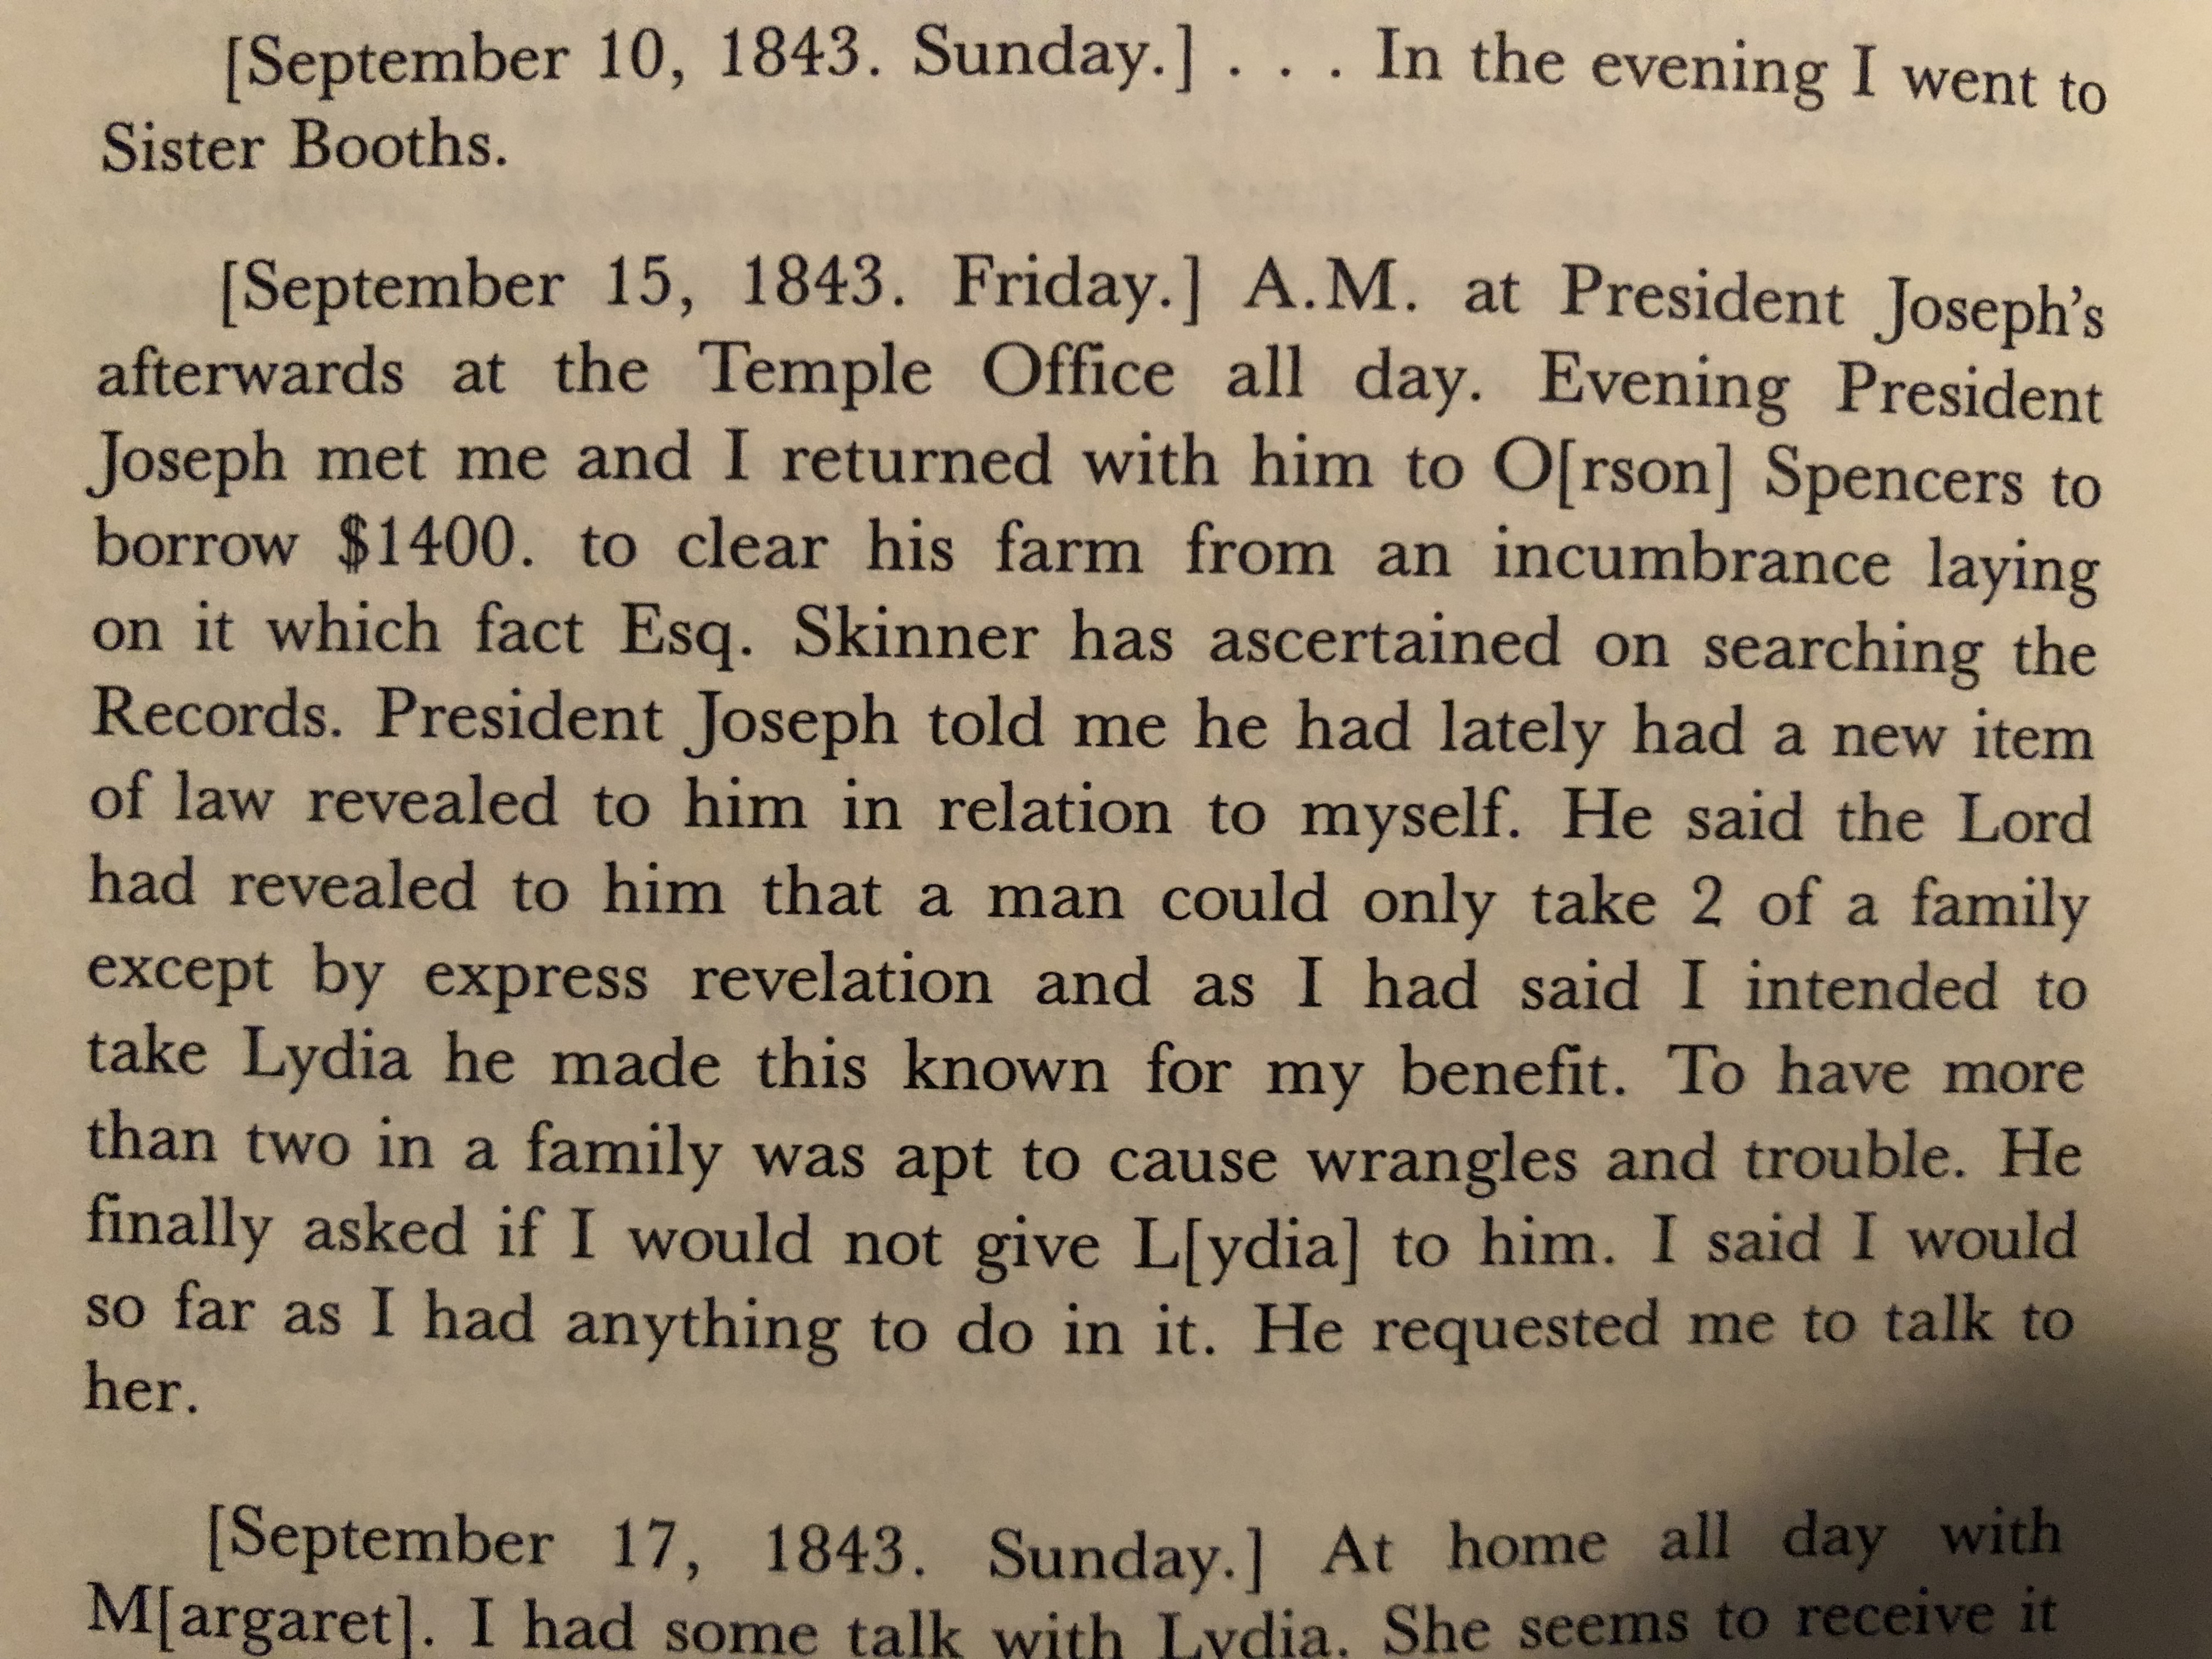
\includegraphics[width=1\linewidth]{2018/images/clayton2.jpg}
  \caption{An Intimate Chronicle: The Journals of William Clayton, p. 120}
  \label{fig:clayton2}
\end{figure}

Take it as you will.

History is an interesting to get into. To be able to look and read about the things
that happened around specific events, it brings about more than just a religious
undertone to the story. These were actual people with real feelings and emotions.
People got hurt during things that took place. Other things happened which aren't
publicly established or given light. It is really interesting indeed.